\documentclass[handout, aspectratio=169]{beamer}
\mode<presentation>{}
\usepackage[utf8]{inputenc}
\newcommand{\fl}[1]{\left\lfloor #1 \right\rfloor}
\usepackage{tikz}

\title{MA 105 : Calculus\\ D1 - T5, Tutorial 12}  % change
\author{Aryaman Maithani}
\date[23-10-2019]{23rd October, 2019}               % change
\institute[IITB]{IIT Bombay}
\usetheme{Warsaw}
\usecolortheme{beetle}
\newtheorem{defn}{Definition}
\begin{document}
\begin{frame}
	\titlepage
\end{frame}
\begin{frame}{Sheet 9}                            % change
	(7) We know that the line integral of a continuous vector field along a smooth curve is independent of the parameterisation. (Assuming that the ``direction'' is preserved.) The question given indeed does satisfy these conditions. Hence, we may choose any parameterisation of our choice.\\
	\uncover<2->{Let $c:[-1, 1] \to \mathbb{R}^2$ be defined as $c(t) := (t, t^2).$ }\\
	\uncover<3->{Then, the required line is integral is given as }\\
	\uncover<4->{\[\int_{-1}^{1} \mathbf{f}(c(t))\cdot c'(t) dt .\] }\\
	\uncover<5->{We compute $c'(t) = (1, 2t).$ }\\
	\uncover<6->{\[\text{Thus,} \int_{-1}^{1} \mathbf{f}(c(t))\cdot c'(t) dt = \int_{-1}^{1} (2t^5 - 4t^4 - 2t^3 + t^2) dt \] }
	\uncover<7->{\[=-\dfrac{14}{15}\] }
\end{frame}
\begin{frame}{Sheet 9}
	(9) Let us parameterise the curve $C$ as $c(t) := \left(x(t), y(t)\right) := (a\cos t, a\sin t)$ for $t \in [-\pi, \pi].$\\
	\uncover<2->{Note that this does parameterise the curve in the desired direction. }\\
	\uncover<3->{With this parameterisation, we now get: }
	\uncover<4->{\[\oint_C \frac{x+y}{x^2 + y^2}dx = \int_{-\pi}^{\pi} \left(\frac{\cos t + \sin t}{a}\right)x'(t) dt = -\int_{-\pi}^{\pi} (\cos t + \sin t)\sin t dt.\] }\\
	\uncover<5->{Similarly, we get that }
	\uncover<6->{\[\oint_C \frac{x-y}{x^2 + y^2}dy = \int_{-\pi}^{\pi} \left(\frac{\cos t - \sin t}{a}\right)y'(t) dt = \int_{-\pi}^{\pi} (\cos t - \sin t)\cos t dt.\] }
\end{frame}
\begin{frame}{Sheet 9}
	Hence, our required integral can now be evaluated as follows:
	\begin{align*}
		\uncover<2->{\oint_C \frac{x+y}{x^2 + y^2}dx - \oint_C \frac{x-y}{x^2 + y^2}dy &= -\int_{-\pi}^{\pi} (\cos t + \sin t)\sin t dt - \int_{-\pi}^{\pi} (\cos t - \sin t)\cos t dt }\\~\\
		\uncover<3->{ &= -\int_{-\pi}^{\pi} 1 dt}
		\uncover<4->{ = -2\pi }
	\end{align*}
\end{frame}
\begin{frame}{Sheet 9}
	(10) It can verified that the given curve can be parameterised as follows:\\
	\uncover<2->{$c(t) := (x(t), y(t), z(t)) := (\cos t, \sin t, \cos t\sin t)$ for $t \in [-\pi, \pi].$ }\\
	\uncover<3->{Once again, it can be seen that this respects the direction given. }\\~\\
	\uncover<4->{Also, $(x'(t), y'(t), z'(t)) = (-\sin t, \cos t, \cos 2t).$ }\\
	\uncover<5->{Hence, we can now evaluate our integral as follows: }
	\begin{align*}
		\uncover<6->{\oint_C ydx + zdy + xdz &= \int_{-\pi}^{\pi} [\sin t(-\sin t) + \cos t\sin t(\cos t) + \cos t(\cos 2t)] dt }\\
		\uncover<7->{ &= \int_{-\pi}^{\pi} (-\sin^2 t) dt + 0  }\\
		\uncover<8->{ &= -\pi }
	\end{align*}
\end{frame}
\begin{frame}{Sheet 10}
	(1) We shall assume that the path given in the question is defined for $t \in [0, 2\pi].$\\
	\uncover<2->{For $t \in [0, 2\pi],$ let }
	\uncover<2->{\[s(t) := \int_{0}^{t} \|\mathbf{r}'(u)\| du. \] }\\
	\uncover<3->{Note that $\mathbf{r}'(t) = -a\sin t \mathbf{i} + a\cos t\mathbf{j} + c\mathbf{k}$ }\uncover<4->{and thus, $\|\mathbf{r}'(t)\| = \sqrt{a^2 + c^2}.$ }\\
	\uncover<5->{This gives us that $s(t) = \sqrt{a^2 + c^2}t.$ }\\
	\uncover<6->{The above is clearly a strictly increasing differentiable function. }\\
	\uncover<7->{Let $h:[0, l(\mathbf{r})] \to [0, 2\pi]$ be its inverse. }\\~\\
\end{frame}
\begin{frame}{Sheet 10}
	\uncover<1->{That is, $h(u) = \dfrac{u}{\sqrt{a^2 + c^2}}.$ }\uncover<2->{It can be seen that $h$ is differentiable and its derivative does not vanish on $[0, l(\mathbf{r})].$ }\\
	\uncover<3->{Now, we define $\tilde{\mathbf{r}}(s) := \mathbf{r}(h(s))}
	\uncover<4->{= a \cos\left(\frac{s}{\sqrt{a^2 + c^2}}\right) \mathbf{i}+a \sin\left(\frac{s}{\sqrt{a^2 + c^2}}\right) \mathbf{j}+c\left(\frac{s}{\sqrt{a^2 + c^2}}\right) \mathbf{k}$ for $s \in [0, l(\mathbf{r})].$}\\
	\uncover<5->{ This is desired arc length parameterisation. }
\end{frame}
\begin{frame}{Sheet 10}
	(4) The only thing to check in this question is whether the question is actually correct.\\
	\uncover<2->{It can be verified that the curve given indeed is smooth. }\\
	\uncover<3->{Moreover, the end points given do actually lie on the path. }\\
	\uncover<4->{Also, the scalar field $(x, y) \mapsto x^2 - y^2$ is a smooth scalar field defined on $\mathbb{R}^2.$ }\\~\\
	\uncover<5->{Thus, we simply get that $\displaystyle\int_C\nabla(x^2 - y^2)\cdot d\mathbf{r} = (2^2 - 8^2) - (0^2 - 0^2) = -60,$ }\\~\\
	\uncover<6->{by FTC for Line Integrals (Part II)}
\end{frame}
\begin{frame}{Sheet 10}
	(5) Note that the square mentioned is the following:
	\uncover<2->{ 
	\begin{figure}
		\centering
		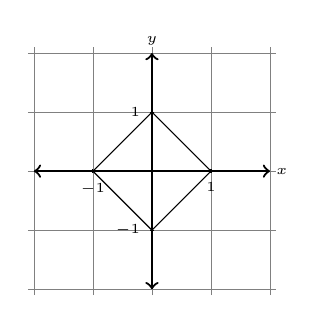
\begin{tikzpicture}[scale = 0.75]
			\draw[step=1cm,gray,very thin] (-2.1,-2.1) grid (2.1,2.1);
			\draw[thick,->] (0,0) -- (2,0);
			\draw[thick,->] (0,0) -- (0, 2);
			\draw[thick,->] (0,0) -- (-2,0);
			\draw[thick,->] (0,0) -- (0, -2);
			\node[] at (2.2, 0) {\tiny $x$};
			\node[] at (0, 2.2) {\tiny $y$};
			\foreach \x in {-1, 1}
   \draw (\x cm,1pt) -- (\x cm,-1pt) node[anchor=north] {\tiny $\x$};
\foreach \y in {-1, 1}
    \draw (1pt,\y cm) -- (-1pt,\y cm) node[anchor=east] {\tiny $\y$};

    \draw[] (1, 0) -- (0, 1) -- (-1, 0) -- (0, -1) -- cycle;

		\end{tikzpicture}
	\end{figure}
	}
	\uncover<3->{This is precisely the square given by $|x| + |y| = 1$ for $(x, y) \in \mathbb{R}^2.$ }\\
\end{frame}
\begin{frame}{Sheet 10}
	\uncover<1->{Thus, our line integral is simply $\displaystyle\oint_Cdx+dy.$ }\\
	\uncover<2->{The above can be written as $\displaystyle\oint_C \nabla(x + y)\cdot d\mathbf{r}.$}
	\uncover<3->{ As $C$ is a closed path, we get $0.$ }\\
	\uncover<4->{(Note that $C$ isn't smooth itself but rather, it is piecewise smooth. Thus, we can't directly appeal to the fundamental theorem but rather, we can break it up into its smooth components and then apply the theorem piecewise.) }
\end{frame}
\begin{frame}{Sheet 10}
	(9) The verification of $\dfrac{\partial}{\partial y}f_1(x, y) = \dfrac{\partial}{\partial x}f_2(x, y)$ can be done easily.\\
	\uncover<2->{Now, recall that $\mathbf{F}$ is a gradient of a scalar field on $S$  } \uncover<3->{ $\iff$ line integrals of $\mathbf{F}$ are path-independent in $S$  } \uncover<4->{ $\iff$ the line integral of $\mathbf{F}$ along every closed path that lies in $S$ is zero.}\\
	\uncover<5->{We shall show that $\mathbf{F}$ is not a gradient of a scalar field on $S$ by showing that the third condition is not true. }\\
\end{frame}
\begin{frame}{Sheet 10}
	\uncover<1->{Indeed, consider the path $\mathbf{\gamma}:[-\pi, \pi]\to\mathbb{R}^2$ given as $\gamma(t) := (\cos t, \sin t).$ }\uncover<2->{Then, $\mathbf{\gamma}$ is indeed a closed path which lies in $S.$ }\\
	\uncover<2->{Now, we compute $\displaystyle\oint_\gamma \mathbf{F}\cdot d\mathbf{s}.$ }
	\begin{align*}
		\uncover<3->{\oint_\gamma \mathbf{F}\cdot d\mathbf{s} &= \int_{-\pi}^{\pi} \sin^2t + \cos^2 t dt  }\\
		\uncover<4->{ &= \int_{-\pi}^{\pi} 1 dt  }	\uncover<5->{ = 2\pi } \uncover<6->{{\color[rgb]{1, 0, 0} \neq 0.} }
	\end{align*}
	\uncover<7->{ Thus, we have shown that $\mathbf{F}$ cannot be the gradient of a scalar field on $S.$}
\end{frame}
	
\begin{frame}{Sheet 10}
	\uncover<1->{This shows us that curl being zero is not a sufficient condition for a field to be a gradient field. }\\
	\uncover<2->{(Technically, we can't talk about curl as this is not a 3D vector field but it can easily be extended to one with our domain then being $(\mathbb{R}^2\setminus\{(0, 0)\})\times\mathbb{R} \subset \mathbb{R}^3.$)}\\
	\uncover<3->{However, later in the course, we'll see a condition on the ``geometry'' of the domain that would indeed imply that curl-free fields are grad fields. }\\~\\
	\uncover<4->{Can you think of examples of when geometry of domain affected the behaviour of functions in the case of one-variable calculus? }	
\end{frame}
\end{document}